\chapter{Herramienta Web. \emph{Back-End}}
\label{backend}

Fijándonos en el diseño preliminar de la figura \ref{fig:herramienta_web_preliminar}, podemos ver que nuestra aplicación Web está dividida en
\emph{front-end} y \emph{back-end}. Esta separación entre módulos es una técnica popular en diseño software. El \emph{front-end} es el encargado de la
capa de presentación, sobre este hablaremos más en el próximo capítulo. En este capítulo nos centraremos en explicar el \emph{back-end}. Este es el
responsable de procesar las peticiones provenientes del \emph{front-end} y devolver le a este la información solicitada. 
\par
El \emph{back-end} es implementado en \emph{PHP}\cite{PHP}. Este es un lenguaje diseñado para desarrollo Web y además es una elección muy popular. Hemos
utilizado \emph{ZendFramework}\cite{ZF}, este es un framework orientado al desarrollo de aplicaciones Web. Junto al framework hemos utilizado
\emph{Apigility}\cite{Apigility}, herramienta que simplifica la creación y mantenimiento de APIs.
\par
El \emph{back-end} tiene un enfoque RPC o \emph{Remote Procedure Call}. Este módulo exporta un conjunto de procedimientos que pueden ser invocados por
el \emph{front-end}. Estos procedimientos realizan tareas específicas sobre un recurso concreto. A lo largo de este trabajo nos referiremos a estos
procedimientos como \emph{servicios RPC}. Un aspecto oportuno destacar es que los servicios RPC son sin estado. Esto quiere decir que la respuesta a
un procedimiento no se ve influenciada por eventos anteriores, esta tan sólo depende de los parámetros proporcionados.
\par
Si nos volvemos a fijar en la figura \ref{fig:herramienta_web_preliminar} podemos ver que en el \emph{back-end} existe la separación entre
\emph{Modelo} y \emph{Controlador}. Esta separación sigue el patrón de diseño MVC\cite{MVCWiki}. Podemos ver que el componente de \emph{Vista} no
existe, en este caso el \emph{front-end} es el componente de \emph{Vista}. Todos los servicios RPC tienen su parte proporcional de \emph{Modelo} y
\emph{Controlador}. La parte de \emph{Modelo} es la encargada de gestionar la información contenida en la base de datos. La parte de
\emph{Controlador} es la encargada de gestionar los mensajes de petición y respuesta.
\par
En este capítulo procederemos a explicar los servicios RPC, pero primero explicaremos algunos aspectos técnicos como la base de datos o el
\emph{ZendFramework}.
\section{Protocolo de comunicación}
	Hemos explicado que entre el \emph{back-end} y \emph{front-end} existe una comunicación, para la que hemos elegido un enfoque RPC. Siendo la
	aplicación que desarrollamos una aplicación Web es de esperar que el protocolo utilizado para la comunicación entre los dos módulos sea
	\emph{HTTP}. En este protocolo se puede diferenciar entre dos tipos de mensajes, mensajes de petición y de respuesta. En nuestra aplicación el
	\emph{front-end} envia mensajes de petición al \emph{back-end}. Los mensajes de petición especifican un campo URL, este campo es muy
	importante porque especifica el servicio RPC que se desea invocar. A la URL también son anexados los parámetros necesarios para el
	procedimiento especificado. Los mensajes de respuesta serán discutidos en el capítulo dedicado el \emph{front-end}. Los mensajes de petición
	también especifican un método, que puede ser \emph{GET} o \emph{POST} (o más cosas) dependiendo de si la operación es lectura o escritura.
	Todos los servicios RPC implementados por el \emph{back-end} son servicios de lectura, a excepción de \texttt{nmdbMarkNull}.
\section{ZendFramework y Apigility}
	Para la realización de este trabajo hemos utilizado \emph{ZendFramework}, este es un framework orientado al desarrollo de aplicaciones y servicios
	Web. Basado en \emph{PHP 5.3+} el framework sigue un diseño orientado a objetos. Esta enfocado en la creación de aplicaciones según el patrón MVC,
	ofrece abstracciones para las bases de datos, autenticación y validación de parámetros. El framework también disfruta de una amplia comunidad
	de usuarios. Todas estas ventajas nombradas anteriormente son la razón para elegir este framework en nuestro trabajo.
	\par
	A la hora de abordar un diseño desde cero, el framework ofrece la aplicación esqueleto. Esta aplicación consiste del código mínimo necesario
	para construir una aplicación usando \emph{ZendFramework}, no tiene ninguna funcionalidad y está pensada para ser extendida. En este trabajo hemos
	empezado con esta aplicación esqueleto.
  	\par
	\emph{Apigility} es una herramienta creada por el equipo responsable de \emph{ZendFramework}. Esta puede utilizarse sin necesidad del framework, sin embargo
	se integra muy bien con este. El obejetivo principal de esta es facilitar la creación y mantenimiento de aplicaciones Web. En nuestro caso nos
	ha ayudado a crear los servicios RPC de nuestra aplicación. La herramienta ofrece un entorno gráfico accesible desde un navegador Web, que es
	muy fácil e intuitivo de utilizar.
\section{Bases de datos}
	Tal y como hemos explicado al principio del capítulo la función del \emph{back-end} es  procesar las peticiones del \emph{front-end} y
	responderle con la información solicitada. Esta información es guardada en dos bases de datos. Para la gestión de las bases de datos
	utilizamos \emph{MySql}\cite{MySql}. En la figura \ref{fig:tablas} podemos ver el esquema de las tablas con las que vamos a trabajar.
	\par
	En la tabla \texttt{binTable} guardamos la información de las cuentas de cada canal. Junto a esta información guardamos las lecturas del
	barómetro, las fuentes de alta tensión y la fecha y hora actuales. La resolución de los datos es de un minuto.
	\par
	En la tabla \texttt{CALM\_ori} guardamos el valor global y las correcciones sobre este. La lectura de presión atmosférica también es guardada.
	La resolución de estos datos es también de un minuto.
	\par
	En la tabla \texttt{CALM\_rev} guardamos la revisión de los datos de \texttt{CALM\_ori}. Vemos que la tabla tiene el mismo esquema con dos
	campos adicionales. En estos dos campos se guardan la fecha de última modificación y la versión. Los datos en esta tabla son introducidos por
	un operario. Cuando este encuentra un dato corrupto en los datos originales, puede crear una entrada en esta tabla para señalarlo.
	\par
	La tabla \texttt{binTable} está almacenada en una base de datos con el nombre \texttt{nmdadb}. Las tablas \texttt{CALM\_ori} y
	\texttt{CALM\_rev} están en otra base de datos con el nombre \texttt{nmdb}. En este documento hablaremos a nivel de tablas, muchas veces sin
	tener en cuenta la separación en diferentes bases de datos. En este punto destacamos esta separación para no crear confusión al lector a la
	hora de contrastar el código fuente con este documento. 
	\begin{figure}[h]
		\centering
		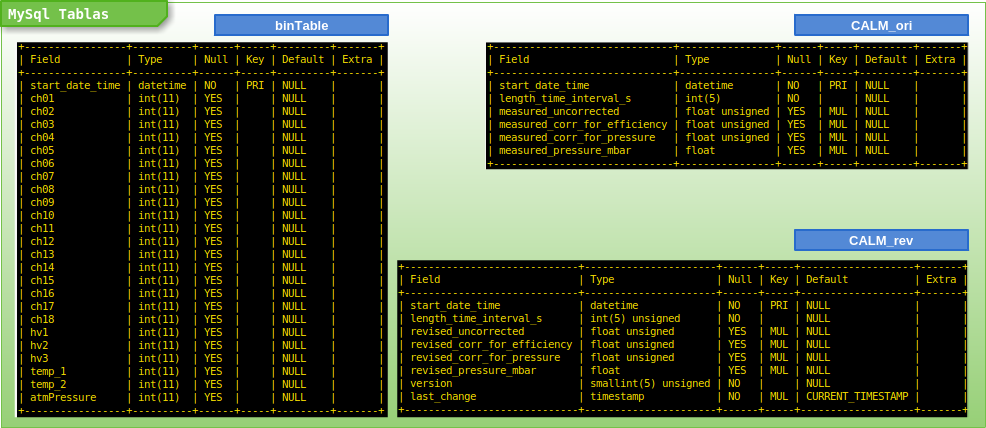
\includegraphics[keepaspectratio, width=1\textwidth]{./img/tablas.png}
		\caption{Esquema de las tablas.}
		\label{fig:tablas}
	\end{figure}
	\par 
	Es interesante destacar que en las tres tablas un existe índice. En los tres casos el elemento indexado es el campo
	\texttt{start\_date\_time}. Este índice es muy útil para la mayoría de consultas que realizamos sobre los datos.
	\par
	\emph{ZendFramework} ofrece abstracciones para las bases de datos que facilitan el trabajo con estas. A continuación presentamos un pequeño ejemplo
	de cómo hacer uso de estas facilidades. \texttt{Zend\textbackslash Db\textbackslash Adapter\textbackslash AdapterInterface} es la abstracción
	que representa un conector a una base de datos. En este ejemplo la variable \texttt{\$this->adapter} es una instancia de esta clase. La
	variable \texttt{resultSet} instancia de la clase \texttt{Zend\textbackslash Db\textbackslash ResultSet\textbackslash ResultSet} es un
	iterable que contiene los datos devueltos por la consulta ejecutada.
	\begin{lstlisting}[style=myPhp]
use Zend\Db\ResultSet\ResultSet;
use Zend\Db\Adapter\AdapterInterface;
//----------------------------------------------
public function interval($start,$finish){
   $sql = "SELECT * FROM binTable WHERE start_date_time "\
           ."between '".$start."' and '".$finish."';";
   $result = $this->adapter->query($sql)->execute();

   $resultSet = new ResultSet;
   $resultSet->initialize($result);
   return $resultSet;}
	\end{lstlisting}
\section{Servicios RPC}
	En esta sección procedemos a explicar todos los servicios RPC que nuestro \emph{back-end} ofrece. Para cada servicio RPC explicamos la
	funcionalidad, la URL que le identifica, los parámetros aceptados, la consulta SQL utilizada y el propósito de este.
	\subsection{\texttt{nmdbOriginalRaw}}
		Este servicio RPC devuelve los datos de la tabla \texttt{CALM\_ori} en un intervalo determinado. Tal y como explicamos en esta tabla
		son guardados los datos globales de la estación, las dos correcciones de estos y los valores de presión atmosférica. Este servicio
		devuelve los datos tal y como están en la base de datos. 
	  	\par
		La URL que identifica a este servicio tiene el siguiente formato.
	  		\begin{center} \texttt{/nmdb/original/raw[/:start][/:finish]}  \end{center} 
		Como vemos el servicio acepta dos parámetros, \texttt{start} y \texttt{finish}. Los parámetros delimitan el intervalo de datos
		devueltos.
		\par
		A continuación podemos ver la consulta SQL utilizada para obtener los datos, dado a la simplicidad de esta no procederemos a discutirla
		más a fondo.
	  		\begin{center} \texttt{SELECT * FROM CALM\_ori 
			  		\\	WHERE start\_date\_time BETWEEN \cc.\$start.\cc AND \cc.\$finish\cc}
			\end{center} 
		Los datos devueltos por este servicio RPC son utilizados para construir un gráfico de líneas.
	\subsection{\texttt{nmdbOriginalGroup}}
		Este servicio RPC es similar al anteriormente descrito en el sentido de que devuelve los datos de la tabla \texttt{CALM\_ori} en un
		intervalo determinado. La diferencia radica en que este no devuelve los datos en crudo, sino que los datos son agrupados y después se
		devuelven valores descriptivos para cada grupo.
		\par
		A continuación podemos ver el formato de la URL que identifica a este servicio.
			\begin{center} \texttt{/nmdb/original/group[/:start][/:finish][/:points]}  \end{center} 
		Los dos parámetros \texttt{start} y \texttt{finish}, al igual que en el servicio anterior, delimitan el intervalo de datos. En este
		servicio estos dos parámetros pueden tener el valor \texttt{all}, de ser así son utilizados todos los datos presentes en la base de
		datos. El parámetro \texttt{points} especifica el número de grupos en los que serán agrupados nuestros datos. 
		\par
		Seguidamente podemos ver parte de la consulta SQL utilizada en este servicio. Esta parte es la encargada de agrupar nuestros datos.
			\begin{center} \texttt{(SELECT CALM\_ori.*,
			  		\\	(UNIX\_TIMESTAMP(start\_date\_time) DIV (.\$interval.)) AS timekey  
				      	\\	FROM CALM\_ori WHERE start\_date\_time BETWEEN \cc.\$start.\cc AND \cc.\$finish.\cc)AS t1  GROUP BY timekey}
			\end{center} 
		Como podemos ver son seleccionados los datos presentes en el intervalo definido por \texttt{\$start} y \texttt{\$finish}. Junto a los
		datos presentes en la tabla \texttt{CALM\_ori} es calculado el campo \texttt{timekey}. Este campo es el utilizado para formar los
		grupos. El \texttt{timekey} es calculado utilizando el valor de la variable \texttt{\$interval}, que a su vez se calcula de la
		siguiente forma:
			\begin{center} \texttt{\$interval =round((\$finish-\$start)/(\$points));}  \end{center} 
		Una vez formados los grupos, para cada uno de ellos se calcula el máximo, mínimo, \emph{open} y \emph{close}. El \emph{open} y
		\emph{close} son la media más la desviación típica y la media menos la desviación típica respectivamente. Estos cuatro valores son
		calculados para el valor global, la corrección por presión y la corrección por eficiencia. Para la presión atmosférica tan sólo es
		calculado el valor medio. Estos datos son utilizados para construir un gráfico \emph{Candlestick}. Sobre este tipo de gráfico
		hablaremos en el siguiente capítulo dedicado al \emph{front-end}.
	\subsection{\texttt{nmdbRevisedRaw}}
		Este servicio es muy similar al \texttt{nmdbOriginalRaw}, la diferencia está en que este devuelve los datos revisados. Para este
		propósito son utilizados los datos de las tablas \texttt{CALM\_ori} y \texttt{CALM\_rev}. La URL utilizada para identificar este
		servicio tiene el siguiente formato.
	  		\begin{center} \texttt{/nmdb/revised/raw[/:start][/:finish]}  \end{center} 
		Los dos parámetros aceptados delimitan el intervalo de datos.
		\par
		En la tabla \texttt{CALM\_rev} son guardados los datos revisados, pero no son guardados todos, tan sólo las entradas que han sido
		modificadas. Por esta razón este servicio también hace uso de \texttt{CALM\_ori} para devolvernos la información completa. A
		continuación podemos ver parte de la consulta SQL utilizada para obtener los datos revisados.
			\begin{center} \texttt{SELECT ori.start\_date\_time,
			  		\\	CASE WHEN rev.start\_date\_time IS NULL THEN ori.measured\_uncorrected ELSE rev.revised\_uncorrected END AS uncorrected 
					\\	FROM CALM\_ori ori LEFT JOIN CALM\_rev rev ON ori.start\_date\_time = rev.start\_date\_time}
			\end{center} 
		La consulta empieza haciendo un \texttt{LEFT JOIN} sobre el campo \texttt{start\_date\_time} de las tablas \texttt{CALM\_ori} y
		\texttt{CALM\_rev}. El \texttt{LEFT JOIN} devuelve todas las entradas de \texttt{CALM\_ori}, con las entradas coincidentes de
		\texttt{CALM\_rev}. La parte correspondiente al \texttt{CALM\_rev} es dejada a \texttt{NULL} si no existe coincidencia. A partir de la
		tabla temporal creada por el \texttt{LEFT JOIN} son seleccionados los datos de \texttt{CALM\_rev} si estos están presentes, en caso
		contario son utilizados lo datos de \texttt{CALM\_ori}. Los datos devueltos por este servicio se utilizan para crear un gráfico
		de líneas.
	\subsection{\texttt{nmdbRevisedGroup}}
		Este servicio es muy similar al {\texttt{nmdbOriginalGroup}, pero este hace uso de los datos revisados. La URL que identifica este
		servicio tiene el siguiente formato.
			\begin{center} \texttt{/nmdb/revised/group[/:start][/:finish][/:points]}  \end{center}
		Los parámetros \texttt{start} y \texttt{finish} delimitan el intervalo de datos. Eventualmente estos dos parámetros pueden tener el
		valor de \texttt{all}, de esta manera son usados todos los datos presentes en la base de datos. El tercer parámetro, \texttt{points},
		especifica el número de grupos en los que queremos agrupar nuestros datos.
		\par
		Para recolectar los datos necesarios la consulta utilizada es una combinación de las utilizadas en los servicios
		\texttt{nmdbOriginalGroup} y \texttt{nmdbRevisedRaw}. Primero se realiza un \texttt{LEFT JOIN} entre las tablas \texttt{CALM\_ori} y
		\texttt{CALM\_rev} para obtener el conjunto de datos revisados. Seguidamente se agrupan los datos de este conjunto y para cada grupo
		se calculan los valores máximo, mínimo, \emph{open} y \emph{close}. Estos datos son utilizados para construir un gráfico
		\emph{Candlestick}.
	\subsection{\texttt{nmdbMarkNull}}
		Este servicio es el más peculiar de todos, ya que los demás servicios son de consulta, mientras que este es de modificación. Uno de
		los propósitos de nuestra aplicación Web es permitir visualizar los datos de la estación y al visualizar un dato corrupto poder
		marcarlo.  Para satisfacer este requisito nuestro \emph{back-end} implementa este servicio que permite marcar como nulo un dato en el
		conjunto de datos revisados. De esta manera pueden ser descartados todos los datos no deseados.
		\par
		A continuación podemos ver la URL utilizada para identificar este servicio.
			\begin{center} \texttt{/nmdb/marknull}  \end{center}
		Como podemos ver este servicio no necesita parámetros. Este servicio acepta un método \texttt{POST}. Los mensajes con método
		\texttt{POST} siempre van acompañados de un campo de datos. Este campo de datos contiene la información del dato que queremos marcar
		como nulo. Eventualmente este campo puede contener un array, de esta forma podemos marcar más de un dato con sólo una llamada al
		servicio.
		\par 
		La consulta SQL utilizada por este servicio es muy simple, esta realiza un \texttt{INSERT} en la tabla \texttt{CALM\_rev}. Si el dato ya
		está presente tan sólo incrementamos la versión actual y modificamos la fecha de última modificación. A continuación podemos ver la
		consulta que estamos discutiendo.
			\begin{center} \texttt{INSERT INTO CALM\_rev 
			  		\\	(start\_date\_time, revised\_uncorrected, revised\_corr\_for\_efficiency, revised\_corr\_for\_pressure, revised\_pressure\_mbar, version, last\_change )
				      	\\	VALUES (\cc.\$start\_date\_time.\cc,null,null,null,null,1,now()) 
				      	\\	on DUPLICATE KEY UPDATE version=version+1, last\_change=now()}
			\end{center} 
	\subsection{\texttt{nmdadbRawData}}
		Este servicio tiene como propósito devolver lo datos crudos de la tabla \texttt{binTable}. La URL utilizada para identificar este
		servicio tiene el siguiente formato. 
	  		\begin{center} \texttt{/nmdadb/rawdata[/:start][/:finish]}  \end{center} 
		Los parámetros \texttt{start} y \texttt{finish} delimitan el intervalo de datos. Para recolectar los datos crudos de la tabla
		\texttt{binTable} este servicio usa una consulta muy simple, que se muestra a continuación.
	  		\begin{center} \texttt{SELECT * FROM binTable 
			  		\\	WHERE start\_date\_time between \cc.\$start.\cc  and \cc.\$finish.\cc}
			\end{center} 
		Los datos devueltos por este servicio son utilizados para construir un gráfico de líneas.
	\subsection{\texttt{nmdadbChannelStats}}
		Este servicio tiene como propósito devolver estadísticas descriptivas para cada canal de la estación. Para este propósito se usan los
		datos de la tabla \texttt{binTable}. Para cada canal son calculados el valor medio, desviación típica, mínimo y máximo. A continuación
		podemos ver la URL utilizada para identificar este servicio.
	  		\begin{center} \texttt{/nmdb/channel/stats[/:start][/:finish]}  \end{center} 
		Los parámetros \texttt{start} y \texttt{finish} delimitan el intervalo de datos. Eventualmente estos dos parámetros pueden tener el
		valor \texttt{default}, en este caso el intervalo es el último mes con datos. 
		\par
		A continuación podemos ver parte de la consulta utilizada para recolectar los datos devueltos por este servicio.
	  		\begin{center} \texttt{select 'ch01' as n1, ch01, avg(ch01) as avg\_ch01, std(ch01) as std\_ch01, max(ch01) as max\_ch01, min(ch01) as min\_ch01
			  		\\	from(select * from  binTable where start\_date\_time between \cc.\$start.\cc and \cc.\$finish.\cc order by start\_date\_time desc)as t1}
			\end{center} 
		Los datos generados por este servicio son utilizados para crear un gráfico \emph{Candlestick} y también son presentados en una tabla.
	\subsection{\texttt{nmdadbChannelHistogram}}
		Este servicio devuelve un histograma de la distribución de cuentas para los 18 canales. Para cumplir con dicho propósito este servicio
		utiliza los datos de la tabla \texttt{binTable}. A continuación podemos ver la URL utilizada para identificar este servicio.
	  		\begin{center} \texttt{/nmdb/channel/histogram[/:start][/:finish]}  \end{center} 
		Al igual que en los otros servicio los parámetros \texttt{start} y \texttt{finish} delimitan el intervalo de datos usados para
		construir el histograma. Eventualmente estos dos parámetros pueden tener el valor de \texttt{default} y en este caso son utilizados los
		datos del último mes.
		\par
		Seguidamente podemos ver la consulta utilizada para construir el histograma devuelto por este servicio.
	  		\begin{center} \texttt{select chh as num, count(chh) as val from (select ch div 5 as chh  from 
				      	\\	(select .\$channel. as ch from binTable where start\_date\_time between \cc.\$start.\cc and \cc.\$finish.\cc) as t1) as t2 group by chh order by num}
			\end{center} 
		La consulta calcula el histograma para un único canal, especificado por la variable \texttt{\$channel}. Para construir el histograma de
		los 18 canales esta consulta es invocada múltiples veces. En esta consulta tenemos que agrupar por el número de cuentas, campo que no está
		indexado. Esto hace que esta tarde bastante más tiempo que las otras, por lo tanto no es recomendable invocarla con mucha
		frecuencia sobre conjuntos muy grandes.
